\section{Version-2 replication results}

The 216 runs completed 510 calls and 707,090 tokens, with 0 infrastructure or protocol errors. Call accounting was complete; tokens were not estimated. 

\subsection{Main comparison: same tasks and model}

\begin{center}\small
\setlength{\tabcolsep}{4pt}
\begin{tabularx}{\linewidth}{@{}Xrrrrr@{}}
\toprule Configuration & Strict & SQL norm. & Tokens & s/task & Calls \\ \midrule
Single agent & 19/24 & 23/24 & 1,160 & 4.62 & 24 \\
Sequential & 20/24 & 24/24 & 3,343 & 12.47 & 72 \\
Parallel & 19/24 & 22/24 & 3,480 & 7.69 & 72 \\
Hierarchical & 18/24 & 22/24 & 4,532 & 11.13 & 96 \\
Reflexive & 20/24 & 24/24 & 2,527 & 9.54 & 54 \\
SAGE-CREH & 23/24 & 23/24 & 1,765 & 7.34 & 38 \\
\bottomrule
\end{tabularx}\end{center}


Each row contains 24 runs. Tokens and seconds are per-task means; calls are the condition total. SQL norm. is a secondary format metric, not answer repair.

\begin{center}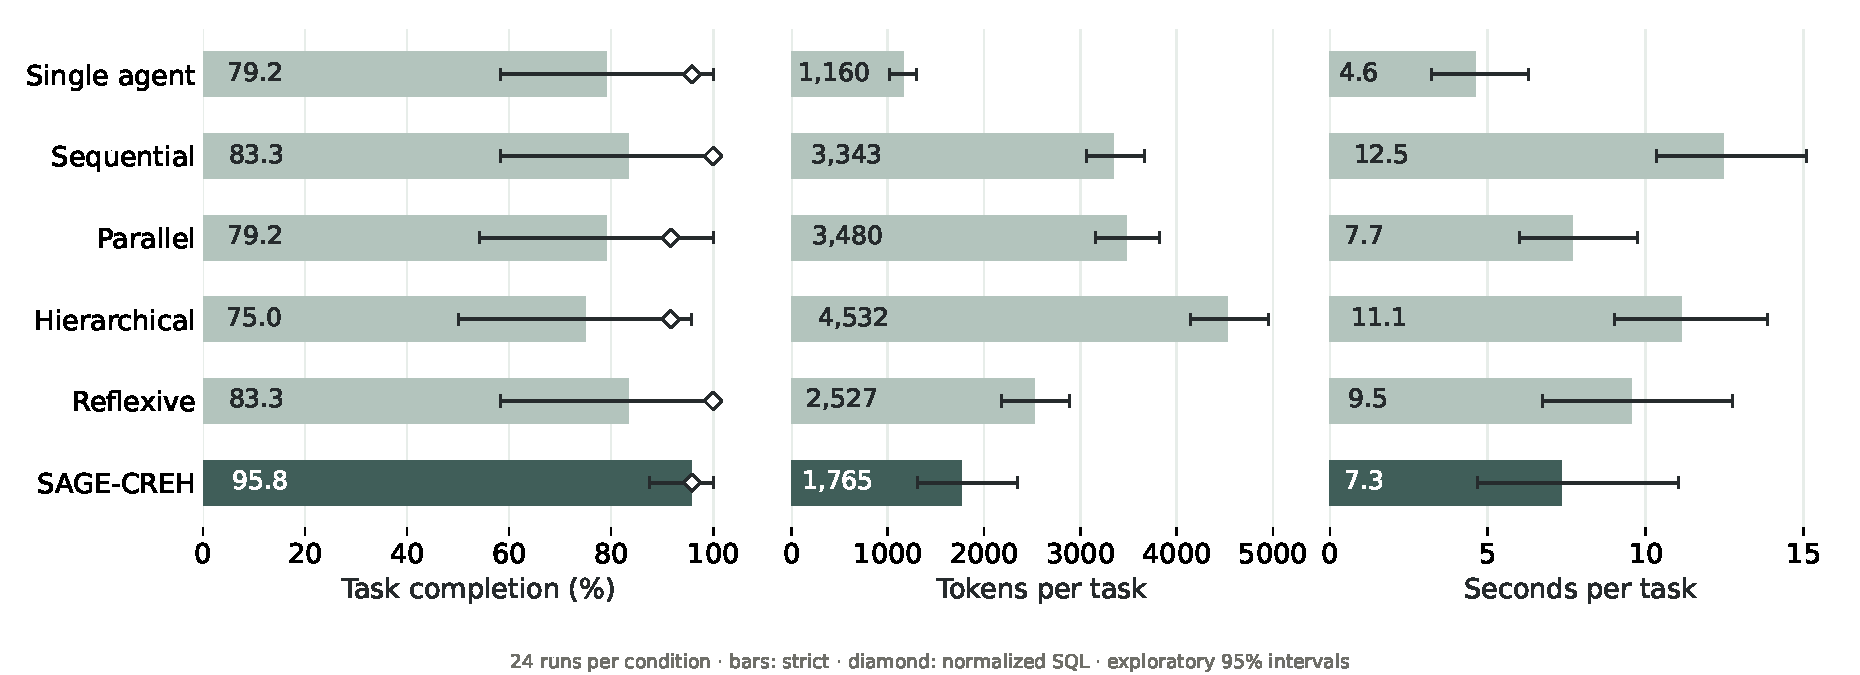
\includegraphics[width=\linewidth]{../../results/analysis-v2/comparison-en.pdf}\end{center}

Strict-completion bars and normalized-SQL diamonds. Task-cluster 95\% percentile intervals do not establish a general architecture ranking.

\subsection{Completion by task family}

\begin{center}\small\begin{tabularx}{\linewidth}{@{}Xrrrrrr@{}}\toprule
Family & Single & Seq. & Par. & Hier. & Refl. & SAGE \\ \midrule
Ledger & 4 / 4 & 4 / 4 & 4 / 4 & 4 / 4 & 4 / 4 & 3 / 3 \\
Calendar & 3 / 3 & 4 / 4 & 4 / 4 & 2 / 2 & 4 / 4 & 4 / 4 \\
Dependencies & 4 / 4 & 4 / 4 & 2 / 2 & 4 / 4 & 4 / 4 & 4 / 4 \\
Selection & 4 / 4 & 4 / 4 & 4 / 4 & 4 / 4 & 4 / 4 & 4 / 4 \\
Memory & 4 / 4 & 4 / 4 & 4 / 4 & 4 / 4 & 4 / 4 & 4 / 4 \\
SQL & 0 / 4 & 0 / 4 & 1 / 4 & 0 / 4 & 0 / 4 & 4 / 4 \\
\bottomrule\end{tabularx}\end{center}

Each cell: strict successes / normalized-SQL successes, both out of four family runs (two tasks times two repetitions). Outside SQL the metrics are identical.

\subsection{Skill-loading and delegation controls}

\begin{center}\small
\setlength{\tabcolsep}{4pt}
\begin{tabularx}{\linewidth}{@{}Xrrrrr@{}}
\toprule Configuration & Strict & SQL norm. & Tokens & s/task & Calls \\ \midrule
Hierarchical & 18/24 & 22/24 & 4,532 & 11.13 & 96 \\
Hierarchy + 10 skills & 20/24 & 22/24 & 8,578 & 10.62 & 96 \\
SAGE-CREH & 23/24 & 23/24 & 1,765 & 7.34 & 38 \\
SAGE without delegation & 21/24 & 21/24 & 1,110 & 5.93 & 24 \\
SAGE + 10 skills & 22/24 & 22/24 & 2,966 & 6.38 & 34 \\
\bottomrule
\end{tabularx}\end{center}


SAGE without delegation retains its proposer and instructions, removing only the second solver and review. SAGE with ten skills retains the policy and changes instruction loading. Original controls include a description catalog absent from SAGE; do not attribute every difference to topology.

\subsection{Paired token and time differences}

\begin{center}\footnotesize\setlength{\tabcolsep}{3pt}\begin{tabularx}{\linewidth}{@{}Xrrrr@{}}\toprule
Comparison & Token change (\%) & 95\% CI & Seconds difference & 95\% CI \\ \midrule
Single agent & +52.2 & [15.9, 95.3] & +2.73 & [1.20, 4.97] \\
Sequential & -47.2 & [-61.5, -29.5] & -5.13 & [-6.29, -3.77] \\
Parallel & -49.3 & [-62.3, -33.8] & -0.35 & [-1.73, 1.52] \\
Hierarchical & -61.1 & [-71.4, -48.5] & -3.79 & [-5.25, -2.30] \\
Reflexive & -30.2 & [-51.8, -3.5] & -2.20 & [-5.33, 0.50] \\
SAGE without delegation & +59.1 & [21.3, 99.0] & +1.42 & [0.46, 2.58] \\
SAGE + 10 skills & -40.5 & [-49.7, -29.6] & +0.96 & [-0.49, 2.94] \\
\bottomrule\end{tabularx}\end{center}

Each row is SAGE minus the indicated configuration; token percentage change is 100(SAGE/control $-1$). Negative values favor lower SAGE consumption or time. Exploratory intervals use 10000 paired task-cluster draws.

\subsection{Executed routes and revision outcomes}

SAGE-CREH. Direct: 13; Parallel agreement: 5; Parallel adjudication: 3; Selective review: 3. Relative to the first candidate: 5 corrections and 0 regressions in strict completion.

SAGE without delegation. Direct: 24. Relative to the first candidate: 0 corrections and 0 regressions in strict completion.

SAGE + 10 skills. Direct: 15; Parallel agreement: 7; Parallel adjudication: 1; Selective review: 1. Relative to the first candidate: 2 corrections and 0 regressions in strict completion.

This inspection uses the evaluator after execution and never fed the routing policy. A correction may concern formatting. Per-run details are retained.

\subsection{Development: excluded from replication}

Serial: 9/10; 1,606.7 tokens and 9.07 mean seconds.

Parallel: 10/10; 1,628.4 tokens and 8.11 mean seconds.

The parallel policy was selected for higher completion under the prior rule. Development used 32,351 tokens in 28 calls and 20 runs. This cost is reported separately and excluded from replication means.

The sole success separating candidates occurred on calendar task DEV22: both policies used the same direct path, without risk or review. Generation variability can explain this difference; it does not establish a causal advantage of parallelism. Selection is retained under the prior rule, not reinterpreted as proof of superiority.
